\subsubsection{Resultados del análisis de latencia}

\begin{figure}[ht]
    \centering
    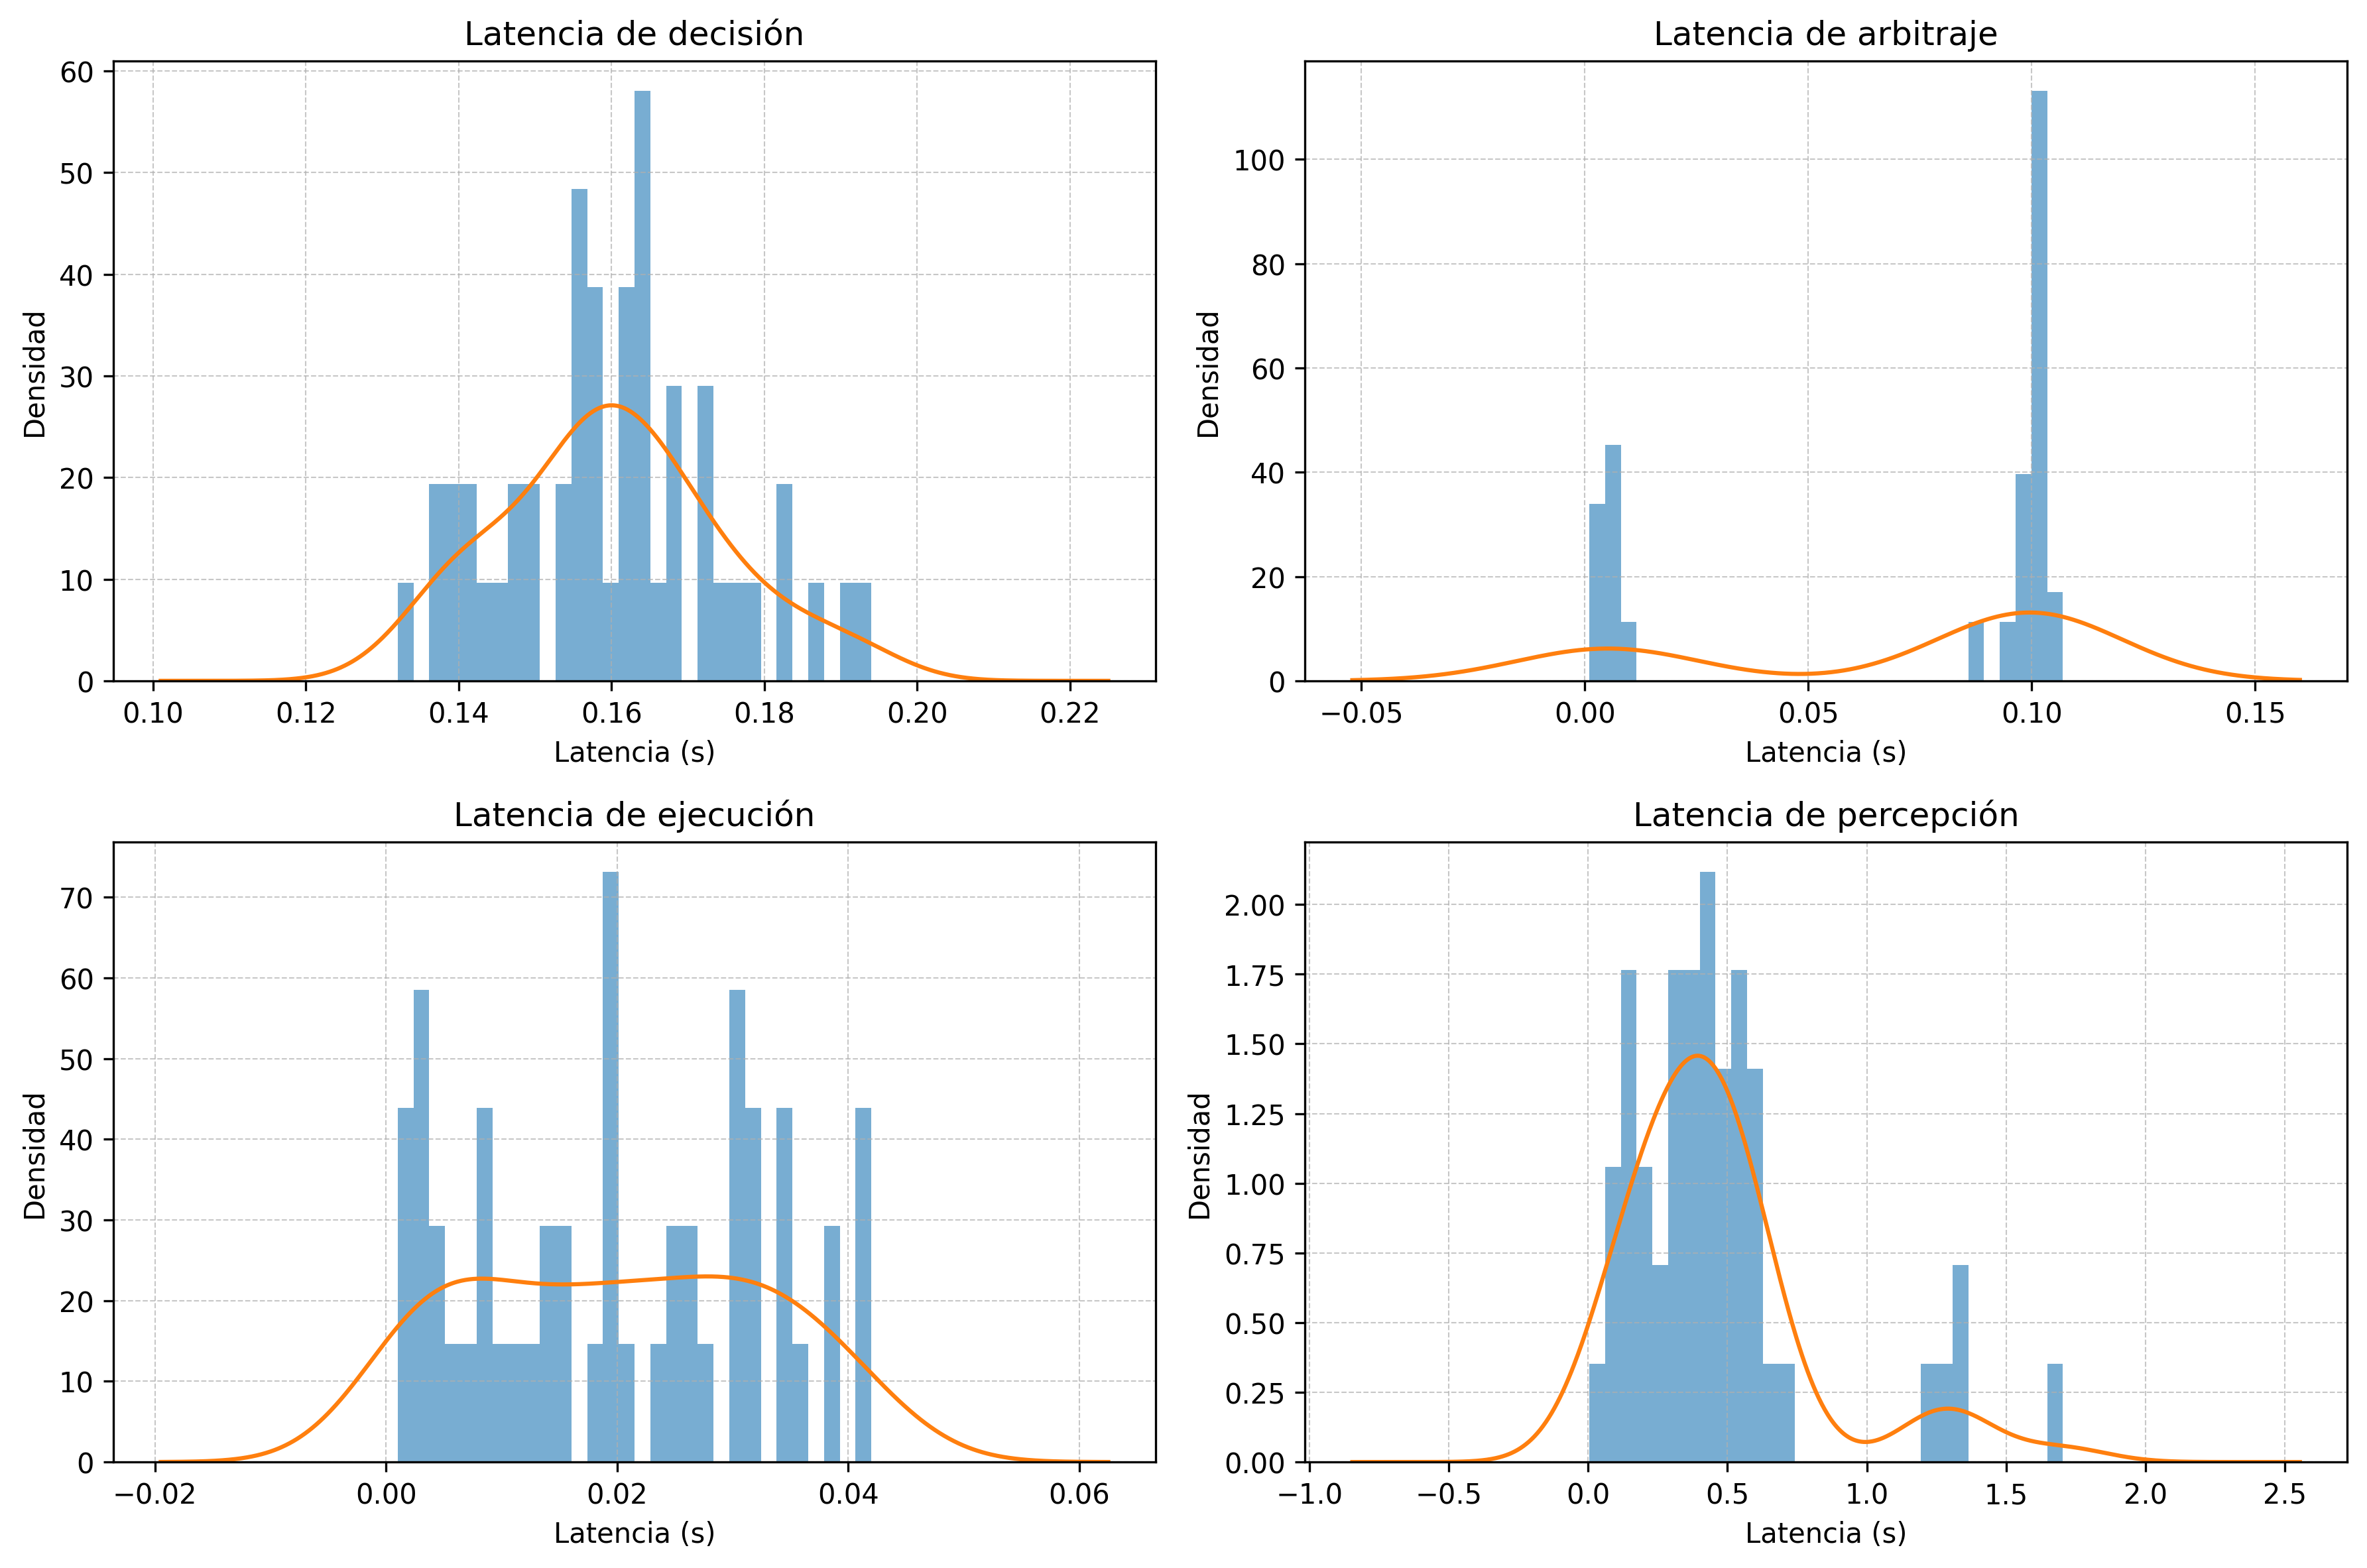
\includegraphics[width=0.9\linewidth]{figures/subsystem_latency_density_distribution.png}
    \caption{Distribución de latencias por subsistema.}
    \label{fig:subsystem_latency_density_distribution}
\end{figure}

\begin{figure}[ht]
    \centering
    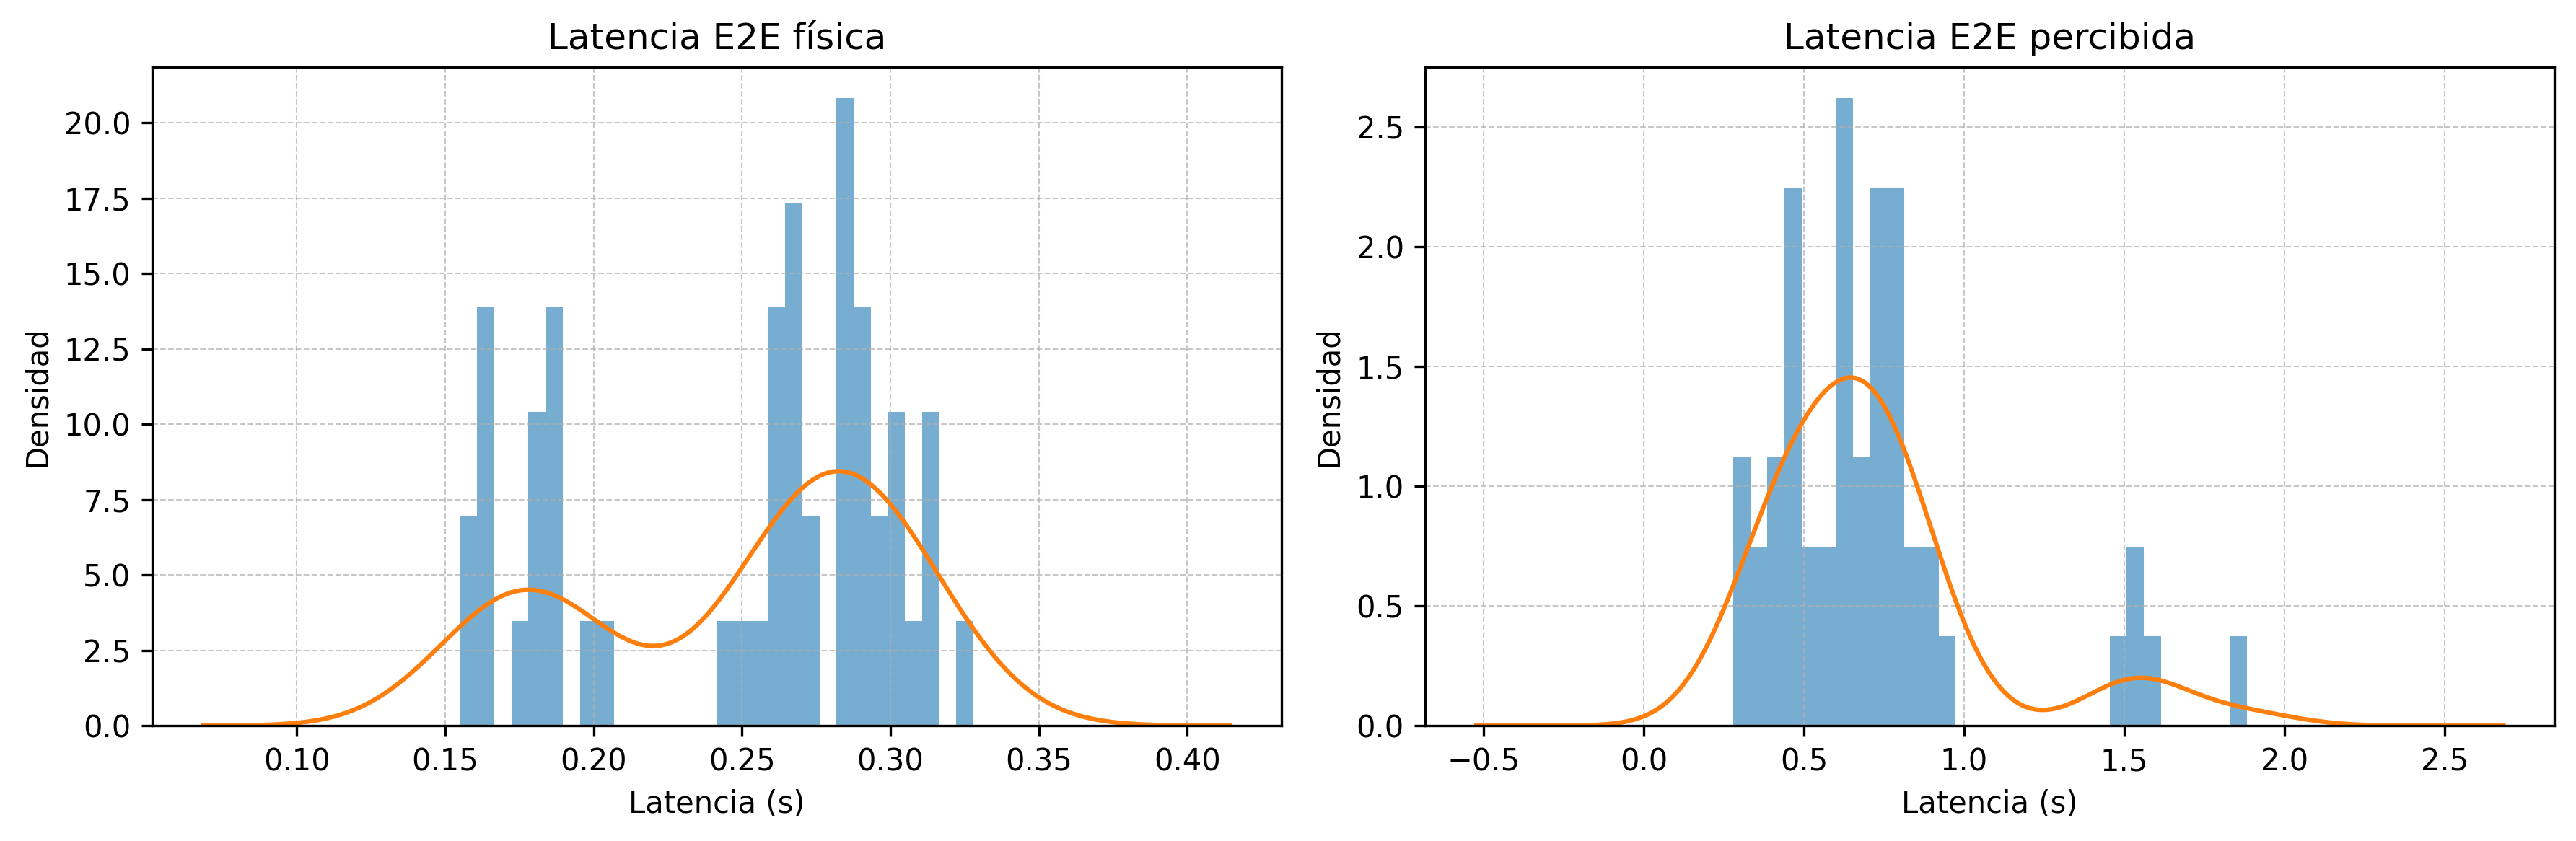
\includegraphics[width=0.9\linewidth]{figures/e2e_latency_density_distribution.png}
    \caption{Distribución de densidad de la latencia end-to-end.}
    \label{fig:e2e_latency_density_distribution}
\end{figure}

\begin{figure}[ht]
    \centering
    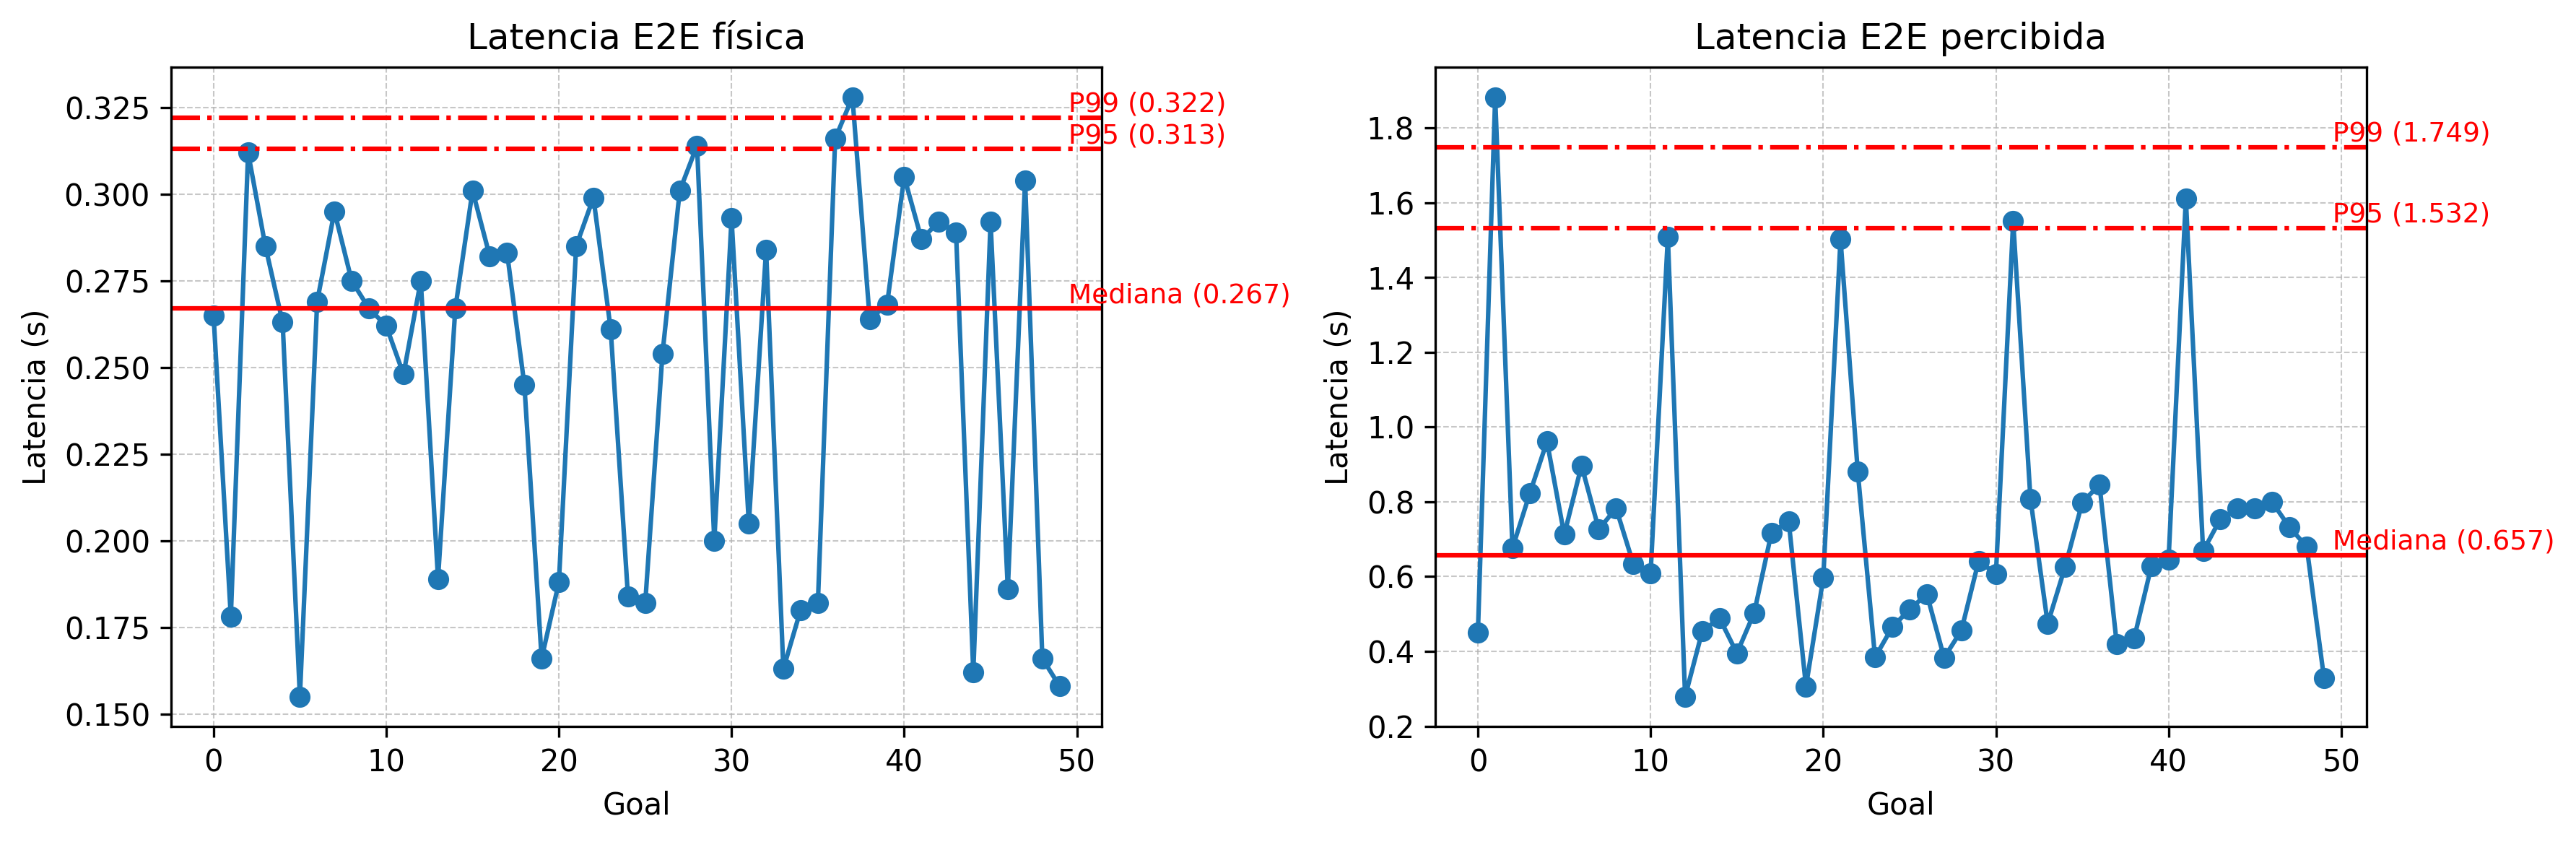
\includegraphics[width=0.9\linewidth]{figures/e2e_latency_per_goal.png}
    \caption{
    Evolución de la latencia end-to-end por objetivo.}
    \label{fig:e2e_latency_per_goal}
\end{figure}


\begin{figure}[ht]
    \centering
    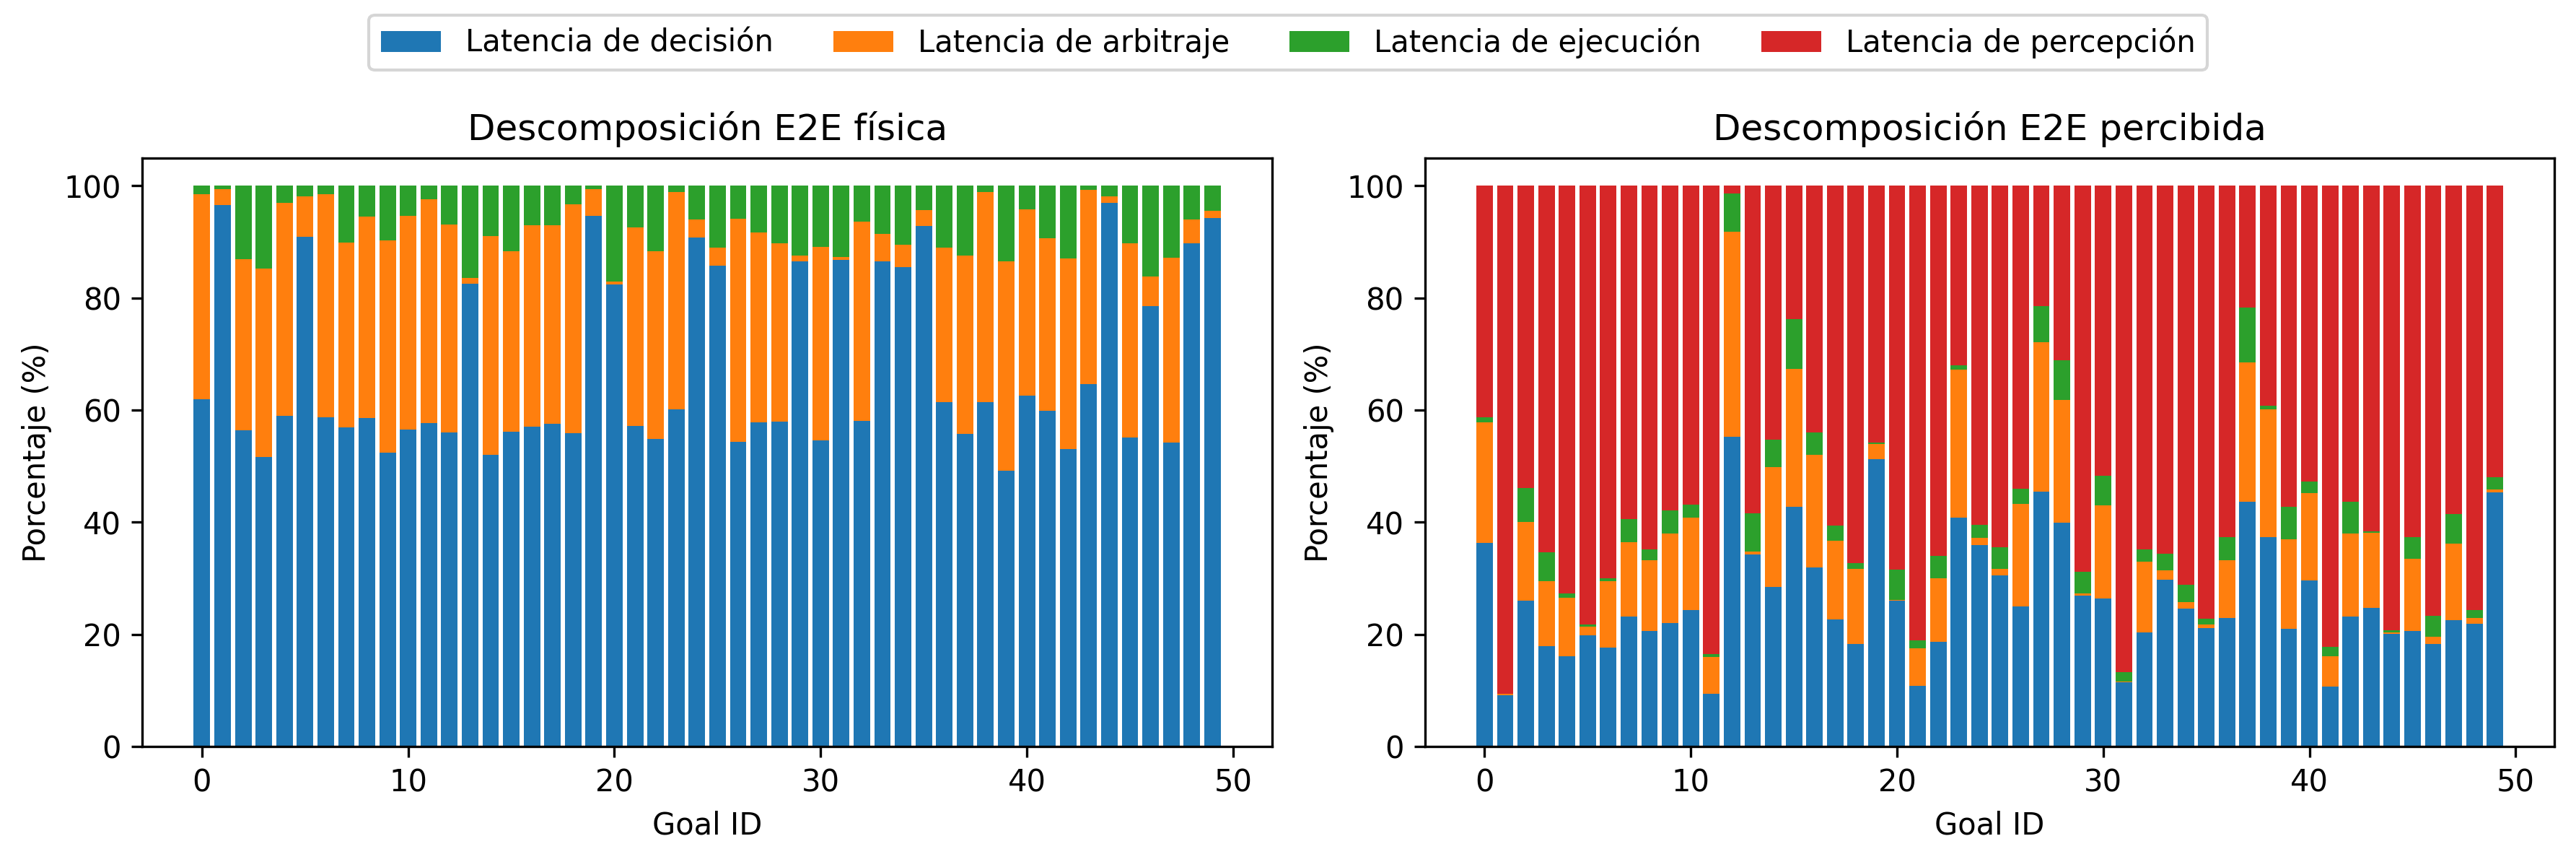
\includegraphics[width=0.9\linewidth]{figures/e2e_latency_decomposition.png}
    \caption{
    Descomposición de la latencia end-to-end de cada objetivo en latencias de los subsistemas.}
    \label{fig:e2e_latency_decomposition}
\end{figure}

\begin{table}[ht]
    \centering
    \small
    \begin{tabular}{lcccccc}
    \hline
    \textbf{Métrica} & \textbf{$L_{decision}$} & \textbf{$L_{arbitraje}$} & \textbf{$L_{ejecucion}$} & \textbf{$L_{percepcion}$} & \textbf{$L_{E2E fisica}$} & \textbf{$L_{E2E percibida}$} \\
    \hline
    Media     & 0.1602 & 0.0693 & 0.0200 & 0.4684 & 0.2495 & 0.7179 \\
    Desv. std & 0.0143 & 0.0446 & 0.0127 & 0.3502 & 0.0531 & 0.3457 \\
    Mínimo    & 0.1320 & 0.0010 & 0.0010 & 0.0040 & 0.1550 & 0.2790 \\
    P50       & 0.1605 & 0.0990 & 0.0200 & 0.4180 & 0.2670 & 0.6570 \\
    P90       & 0.1784 & 0.1011 & 0.0362 & 0.7499 & 0.3041 & 1.0151 \\
    P95       & 0.1852 & 0.1031 & 0.0401 & 1.2951 & 0.3131 & 1.5316 \\
    P99       & 0.1925 & 0.1055 & 0.0415 & 1.5281 & 0.3221 & 1.7487 \\
    Máximo    & 0.1940 & 0.1070 & 0.0420 & 1.7040 & 0.3280 & 1.8820 \\
    \hline
    \end{tabular}
    \caption{
    Estadísticos descriptivos y percentiles de latencia por subsistema y latencias E2E (en segundos).}
    \label{tab:latency_centralized_stats}
\end{table}

La Figura~\ref{fig:subsystem_latency_density_distribution} muestra la distribución de latencias por subsistema, evidenciando comportamientos diferenciados que reflejan la naturaleza funcional de cada módulo.
El subsistema de decisión presenta una distribución aproximadamente unimodal y relativamente concentrada en torno a 0.16 s, con una dispersión moderada. Este patrón es consistente con un proceso determinista con carga computacional estable, donde la variabilidad observada puede atribuirse principalmente a pequeñas fluctuaciones en la disponibilidad de datos de entrada o planificación interna.
Por el contrario, el subsistema de arbitraje exhibe una distribución claramente multimodal, con agrupaciones bien definidas en distintos rangos de latencia. Este comportamiento no es ruido, sino indicativo de la existencia de múltiples caminos de ejecución o políticas de selección de comandos, lo que sugiere que el coste temporal depende fuertemente del contexto operativo (por ejemplo, complejidad del conflicto a resolver).
El subsistema de ejecución, aunque presenta valores medios muy reducidos (media = 0.0200 s), muestra una distribución irregular y dispersa, sin una forma claramente gaussiana. Esto apunta a un proceso ligero pero sensible a factores externos, como la sincronización con el sistema de control, introduciendo jitter aunque acotado en magnitud.
Finalmente, el subsistema de percepción concentra la mayor complejidad temporal del sistema. Su distribución presenta un núcleo dominante en el rango 0.4--0.6 s, acompañado de eventos aislados de alta latencia que generan una cola pesada. Este patrón es característico de procesos intensivos en computación y dependientes de entrada sensorial, donde la carga varía dinámicamente (por ejemplo, en función de la complejidad del entorno). Los percentiles superiores (P95 = 1.295 s, P99 = 1.528 s) confirman la presencia de episodios de degradación puntual, lo que convierte a este subsistema en el principal contribuyente a la variabilidad global del sistema.
Estos resultados se sintetizan en la Tabla~\ref{tab:latency_centralized_stats}, donde se observa que la variabilidad de la latencia de percepción es del mismo orden que la de la latencia end-to-end percibida, tanto en desviación estándar como en percentiles altos. 
Aunque la latencia end-to-end incorpora contribuciones adicionales de otros subsistemas, la similitud en términos de dispersión indica que el módulo de percepción constituye el principal factor que determina la variabilidad global del sistema.

Por el contrario, la latencia percibida presenta una mayor dispersión y una estructura heterogénea, 
con un núcleo principal en torno a 0.5--0.8 s y la aparición de eventos de alta latencia. La mediana se sitúa en 0.657 s, 
mientras que los valores extremos alcanzan 1.882 s. Los percentiles altos (P95 = 1.531 s, P99 = 1.748 s) evidencian 
la existencia de episodios de degradación temporal claramente diferenciados del comportamiento nominal.

Estos resultados se sintetizan en la Tabla~\ref{tab:latency_centralized_stats}, donde se observa que la variabilidad de la latencia de percepción
es comparable a la de la latencia end-to-end percibida, lo que indica que este subsistema actúa como 
principal fuente de variabilidad del sistema.

Finalmente, la Figura~\ref{fig:e2e_latency_per_goal} muestra la evolución de la latencia end-to-end por objetivo. 
La latencia física presenta variaciones acotadas dentro de un rango estrecho, aunque con cambios irregulares entre objetivos, lo que indica un comportamiento estable en magnitud pero no completamente uniforme.
Por el contrario, la latencia percibida muestra una mayor variabilidad, con oscilaciones pronunciadas y la aparición de picos aislados de alta latencia, coherentes con los valores extremos observados en las distribuciones.

La Figura~\ref{fig:e2e_latency_decomposition} muestra la descomposición porcentual de la latencia end-to-end para cada objetivo.
En el caso de la latencia física, la contribución está dominada por los módulos de decisión y arbitraje, con una participación consistente y estable entre objetivos, mientras que la ejecución presenta un impacto marginal. Este comportamiento refleja un pipeline de control determinista y con baja variabilidad.
Por el contrario, en la latencia percibida se observa un cambio estructural claro: el módulo de percepción pasa a ser el principal contribuyente, alcanzando en numerosos casos más del 70\% de la latencia total. Además, su contribución presenta una elevada variabilidad entre objetivos.
Estos resultados evidencian que el incremento de latencia y variabilidad observado en el sistema no se origina en el pipeline de control, sino en el proceso de percepción, que actúa como principal cuello de botella del sistema.

En conjunto, los resultados indican que la diferencia entre latencia física y percibida no es únicamente de magnitud, 
sino también de naturaleza estadística. Mientras que la primera presenta un comportamiento estable, la segunda está 
caracterizada por una mayor dispersión, asimetría y presencia de eventos extremos, lo que evidencia una fuente de 
variabilidad estructural asociada al proceso de percepción.